\documentclass[journal=jpcafh,manuscript=article]{achemso}
\usepackage[english]{babel}
\usepackage{amsmath}
\usepackage{amsfonts}
\usepackage{amssymb}
\usepackage[T1]{fontenc}
\usepackage[utf8]{inputenc}
\usepackage{lmodern}
\usepackage{graphicx}
\usepackage{epstopdf}
\usepackage[numbers]{natbib}

\graphicspath{ {./images/} }

\SectionNumbersOn

\author{Franz Martinez}
\email{franzmichel.martinez@ucalgary.ca}
\affiliation{Schulich School of Engineering, University of Calgary, Calgary, Alberta, Canada}
\title{Outline--Draft JCP format for: Reactive Force Field for Solid Oxides Containing Lanthanum}

\begin{document}

\begin{abstract}
\textbf{abstract needs to be updated to reflect changes in focus of the paper}


In this work, we perform the parametrization of a reactive force field, ReaxFF, for Lanthanum and its oxides.
We describe the procedure followed and provide results that validate the derived parameters in their ability to describe bulk structures, surfaces, and nanoparticles.
Comparison of our results using ReaxFF and electronic structure methods show good agreement in the reproduction of surfaces energies and bulk modulus, as well as good agreement with experimentally reported results for the latter.
We also show that the resulting force field can capture changes in the crystal structure of Lanthanum and its oxides by reproducing the expected crystal structure at various ranges of temperature as well as reasonable values for the temperatures in which crystal structure phase transitions occurs.
Overall, these results highlight the utility of ReaxFF to study systems containing Lanthanum and its power to predict thermodynamic related processes involving the crystal structure of the system.


\end{abstract}


\section{Introduction}

% introduce lanthanum uses
Lanthanum and Lanthanum oxide are materials involved in various applications involving catalysts, batteries, and medicine \cite{atwood2013rare,he2013preparation}.
Particularly, catalysts based on Lanthanum oxide have shown a good efficiency in the oxidative coupling of methane to form ethane and/or ethylene \textbf{import citation}, or as main components of electro--catalysts used in CO$_2$ conversion to CO \textbf{import citation}.
While the experimental properties of Lanthanum and its oxides are well studied and known \textbf{import citation}, their interaction with other compounds is an area of growing study and interest for advancements in material design involving Lanthanum.

%\emph{need to introduce more about uses of La}

Computational methods are often used together with experimental data to study interaction between atoms and gain an understanding of them.
Quantum mechanical calculations are one of the most used computational methods to resolve the interaction between all electrons and atomic nuclei of a system and are based in solving the Schrödinger equation of a particular system.
However, many of the phenomena of interest involving La, and material design in general, take place between many atoms, making rigorous quantum mechanical calculations unfeasible when many atoms are present in the system.
Alternatively, force fields can be used instead of quantum mechanical calculations when the size of the system makes the latter computationally prohibitive.
Most force fields use parametrized potential energy functions to capture the interaction between atoms of a system and reproduce, to some extent, its high dimensional potential energy surface.
Because these functions are easier to evaluate than their quantum mechanical counterparts, it is possible to model systems of many atoms and capture the dynamics on nanosecond time scales.
At the same time, the major drawback of using force fields is the loss of the accurate quantum mechanical interaction between particles, which is important in Lanthanum due to the complexity introduced by strongly correlated 4f electrons and the high polarizability of the atom.
For this reason, it is critical to have good quality force fields that can reproduce the properties of Lanthanum and its oxides and expand them to study their interactions with other compounds.

Modeling of Lanthanum has been commonly done with general force fields, being UFF the most used \textbf{import citation}, but using this approach has some shortcomings.
General force fields favor transferability and simplicity, an approach that has been very successful for elements in the first rows of the periodic table, but in the case of heavier elements this approach is not enough to capture their behaviour, and specialized force fields need to be developed to improve on the shortcomings of the general force fields.
In particular for La, the behaviour of La$^{3+}$ in aqueous solution is the most studied interaction and has been investigated by various groups using different parametrization strategies \cite{clavaguera2005molecular,duvail2007pair}.
These studies highlight the importance of introducing some form of explicit polarizability and many-body effects to improve the accuracy of the Lanthanum--water interaction.

Another shortcoming of general force fields is the impossibility to describe chemical reactions, which would require modeling explicit bond breaking and formation, historically handled only by quantum mechanical calculations.
However, development of computational techniques and increasing computational power have given rise to the use of reactive force fields \cite{meuwly2019reactive}, where bond breaking and formation is treated by introducing functions describing changes in the bond order of the atoms \textbf{import citation}, or by using valence bond theory \textbf{import citation}, or by explicitly computing the potential energy surface of the system on--the--fly \textbf{import citation}.
Most of these methods are novel, and those involving the computation of the potential energy surface of the system on--the--fly still require a lot of computational resources.
Nonetheless, among these methods ReaxFF \cite{van2001reaxff,chenoweth_reaxff_2008} is a reactive force field that has been used successfully to study reactive events in hydrocarbons \cite{van2001reaxff}, thermal decomposition of zinc-oxide \cite{russo2011atomistic}, H$_2$ on platinum surfaces, oxidation on aluminum surfaces \cite{ludwig2006dynamics}, and hydration on calcium oxide surfaces \cite{manzano_hydration_2012}, just to mention some examples.
ReaxFF is a promising reactive force field, it has room for performance improvements and can be extended to study a wide range of chemical reactions and phenomena \cite{senftle_reaxff_2016}.

The formalism used to develop ReaxFF gives it the ability to describe not only chemical reactions but also interactions between different phases, e.g. solid--liquid, gas--solid, etc. as evidenced by some of the studies cited previously.
In addition, due to the many functions used to capture the interactions between atoms in ReaxFF, some form of polarizability is present in the force field, as well as many-body effects.
For these reasons, ReaxFF is a viable force field for studying phenomena involving crystal structure determination and chemical reactions (e.g. heterogeneous catalysis) of Lanthanum.

Although the current form of ReaxFF has been in development since 2008 \cite{chenoweth_reaxff_2008} and many elements have been parametrized to be used in ReaxFF, transferability between parameters is limited.
Also, because ReaxFF does not build on the concept of atom types, fitting to reference data is somewhat necessary.
For systems containing atoms that are commonly studied, e.g. C, H, O, etc. fitting may be minimal compared to systems where one atom has no previous known parametrization, which is the case for La.

The purpose of this study is to generate a set of parameters for Lanthanum and Lanthanum oxide that can be used for describing their thermodynamic and structural properties, and serve as a base for further development in applications that involve interactions with other materials.
To this end, in the remainder of this paper, we introduce the mathematical form of ReaxFF and a parametrization strategy in Sec.~\ref{sec:reaxff-strategy}; the computational methods used, i.e. electronic structure calculations in Sec.~\ref{sec:dft-details}, and molecular dynamics simulations in Sec.~\ref{sec:md-details}.
Then, we discuss in Sec.~\ref{sec:results-and-discussion} the quality of the newly generated parameters by analyzing the ability of ReaxFF to reproduce a dataset from quantum mechanical calculations.
In the following section Sec.~\ref{sec:applications}, we use the parameters obtained to predict some structural and thermodynamic properties and discuss the results, and we present our concluding remarks in Sec.~\ref{sec:conclusions}

%CO$_2$, electrocatalysts, and solid oxide fuels.\cite{
%habisreutinger_photocatalytic_2013,
%e.benson_electrocatalytic_2009,
%pradeepindrakanti_photoinduced_2009,
%indrakanti_quantum_2009,
%zeng_review_2018,
%yamada_systematic_2018,
%kar_enhanced_2016,
%grimaud_double_2013,
%ni_electrochemical_2012,
%tan_co_2011,
%baniecki_photoemission_2008,
%jia_heterogeneous_2017,
%yin_oxide_2018,
%zheng_review_2017,
%andersson_review_2010,
%beatriz_microwave-assisted_2015}
%
%DFT studies.\cite{tian_dft_2018,
%mayeshiba_strain_2017,
%wang_oxidation_2006,
%li_density_2013,
%liu_influence_2018,
%seo_design_2015,
%evarestov_adsorption_2007,
%pilania_establishing_2012,
%pilania_adsorption_2010,
%zurek_predicting_2015}
%
%Molecular dynamics studies.\cite{wang_coarse-grained_2014}

\section{Computational Methods}

\subsection{ReaxFF and Parameterization Strategy}
\label{sec:reaxff-strategy}

ReaxFF is a force field based on the dynamical computation of the bond-order, which dictates the connectivity between atoms on the fly.
This approach allows ReaxFF to consider bond breaking and formation, and follow the apparition of intermediates during a chemical reaction.
In complex systems this ability proves to be invaluable for following reaction mechanism when the number of atoms are in the order of thousands or higher.\cite{migliorati_development_2017,merinov_reaxff_2014,
raymand_reactive_2008,
shin_development_2015,
van_duin_reaxff_2008,
goddard_development_2006,
hubin_parameterization_2016,
senftle_reaxff_2016,
chenoweth_reaxff_2009,
chenoweth_reaxff_2008,
van_duin_reaxff_2008-1,
liu_reaxff-lg:_2011}

To this end, ReaxFF uses the following energy terms:
\begin{equation}
E = E_{bond} + E_{over} + E_{angle} + E_{tors} + E_{vdW} + E_{coul} + E_{special},
\end{equation}
where $E_{bond}$ is the energy associated with bond formation between atoms and it is function of the bond order; $E_{angle}$ and $E_{torsion}$ are the three-body angle and four-body torsion strains, respectively, which are also dependent of the bond order; $E_{over}$ is an energy penalty that prevents overcoordination of atoms based on atomic valence rules; $E_{coul}$ and $E_{vdW}$ are the coulombic and van der Waals interactions, respectively; and $E_{special}$ are less commonly used energy terms that are used to describe specific properties like lone-pair interactions, conjugation, $C_2$ corrections, hydrogen binding and undercoordination.
For an introduction of the full mathematical form of the various energy terms as well as their parameters refer to the publications from \citet{van2001reaxff} and \citet{chenoweth_reaxff_2008}.

Parametrization of ReaxFF involves generation of a dataset, generally from quantum mechanical calculations, and subsequent fitting of the force field parameters with respect to the dataset by minimizing the error function, $E_f$,
\begin{equation}
E_f = \frac{(x_{i} - x_{ReaxFF,i})^2}{w_i}.
\end{equation}
Where $x_{i}$ is the reference value of a property $x$ (e.g. heat of formation, bond distances, angles, charges, energetic differences, etc.); $x_{ReaxFF,i}$ is the property calculated using ReaxFF; and $w_i$ is a weight, or accuracy, associated to the desired deviation that can be tolerated between both $x_i$ and $x_{ReaxFF,i}$.
In this work the error function minimization is carried out using the CMA-ES force-field optimizer,\textbf{fix citations}\cite{iype_parameterization_2013} part of the ADF package.
Among various methods for parametrizing ReaxFF, CMA-ES has shown to give reliable results independent of the initial guess for the force fields parameters, which in this work is of concern as full parameters for La has not been generated yet.

The parametrization of the force field was performed using various stages.
The first stage of the parametrization involved fitting the La--La parameters of the force field to the following: quantum mechanically calculated equations of state corresponding to three solid phases of La, i.e. double hexagonal close packed (dhcp, $\alpha$-La), face centered cubic (fcc, $\gamma$-La), and body centered cubic (bcc, $\beta$-La); data from the electronic structure calculation of the La$_2$ and La$_3$ molecules were added as well.
At this point, the starting parameters (initial conditions) for La were randomly generated, and various fittings were carried out with different initial conditions
The following stage involved further fitting of the La--La parameters, namely those related to the electrostatic interaction (EEM shielding, EEM electronegativity, and EMM hardness), and the La--O parameters by adding to the dataset Mulliken charges and geometrical information obtained from the optimized structures of the La$_2$O$_3$ cluster, three La$_4$O$_6$ clusters, and one La$_6$O$_9$ cluster.
Also, the equations of state corresponding to two solid structures of La$_2$O$_3$ were computed and added.
In this stage, the La--La parameters obtained from the first stage were kept fixed, and the initial conditions of stage two corresponded to a set of force fields parameters that had the lowest values for the error function in stage one.
As a last stage, all parameters were allowed to vary during the fitting procedure, using as initial conditions the force field parameters that had the lowest values for the error function in stage two.
The best force field for which results are presented in the following sections was the one with the lowest error function value and, also, presenting the lowest error function value for a validation dataset.
The datasets were constructed such that all the quantum mechanical properties calculated were distributed in a 9:1 ratio to form the training and validation datasets.


\subsection{Electronic Structure Calculations for Dataset Generation}
\label{sec:dft-details}

DFT calculations are carried out using Quantum Espresso,\cite{giannozzi_advanced_2017} for all solid structures in bulk or slab form.
These calculations were performed using the pseudo--potentials from the PSlibrary including scalar-relativistic effects for Lanthanum \textbf{put references}.
A value of 75.0 Ry was used for the kinetic energy cutoff, which was tested for convergence ensuring that $\Delta E_{tot} / \Delta E_{cut} <$ 0.01 eV was obtained per atom.
Monkhorst-Pack k-point sampling of the Brillouin zone was chosen to be $4\times4\times4$ for most calculations.
The criterion used involved using a k-point grid of 4 on the edge of a cell between 5 and 8 \AA in length, then to preserve the grid on bigger or smaller cells, the grid was scaled accordingly.
The k-point grids used were also tested using the same criterion from energy convergence to ensure convergence with respect to grid size.

%Because the transition metals present localized electronic density on their d--orbitals with strong correlation, the Hubbard correction is employed to take into account these effects.\textbf{put references}
%Values used for the Hubbard term, U, were taken from \textbf{put values, and justify about not determining their values from linear response theory}

The convergence criterion used for all calculations was of 0.02 eV for the total energy, and in the case of relaxations the maximum force component on each atom had to satisfy being smaller than 0.01 eV/\AA 

Differences in energies and optimized geometries were also obtained from clusters in the gas phase using \emph{Gaussian16} \textbf{put references}.
For these calculations, the B3LYP functional has been used with the aug--cc--pVTZ basis functions for oxygen and for lanthanum the La basis set from the Stuttgart/Dresden group, La(RSC97) \textbf{double check} with a 28--electron ECP \textbf{citation}.
By using this approach, we ensure that the parameters obtained for lanthanum in these calculations are consistent with the way the oxygen parameters were obtained in previous studies.

\subsection{Molecular Dynamics Trajectories Using ReaxFF}
\label{sec:md-details}

For the molecular dynamics simulations using ReaxFF, the system \textbf{specify details for bulk simulations and slabs} ... first is equilibrated using classical molecular dynamics with the UFF force field.
From the equilibrated trajectory at the conditions required \textbf{double check temperature and pressure and change this part}, several points are selected randomly as starting points for the simulation.
This ensures that the system starts from a correct point in equilibrium of the ensemble for the ReaxFF dynamics.

\section{Parametrization Results and Discussion}
\label{sec:results-and-discussion}

\subsection{Equations of State}

Equations of state for hexagonal La, ... La$_2$O$_3$, ... \emph{fill in other crystals} were calculated using DFT, and ReaxFF was parametrized to reproduce these curves to the best possible fit, i.e. using weights of 0.1 to 1.0.
Because the relationship between energy and volume in solids allows to capture the stability of the phase, fitting of these curves give ReaxFF the ability to model accurately the bulk phase of the crystal structures.

\emph{all these results may actually change as the force field gets improved}

The equations of state for the three forms of Lanthanum are presented in Fig.~\ref{fig:laeos}.
The plots show the parabolic behaviour of the equation of state, and that the parametrized ReaxFF can reproduce the results from DFT within an acceptable margin of error for high densities of the crystals, but shows a degradation when volume is increased (low densities), particularly for $\beta$-La.
As for the trends in stability of the three phases, ReaxFF is unable to properly reproduce it.
The reported experimental trend places $\alpha$-La as the most stable phase, followed by $\beta$-La, and then by $\gamma$-La.
In the case of ReaxFF, the predicted most stable phase corresponds to that of the $\gamma$-La, followed by $\beta$-La, and placing $\alpha$-La as the least stable phase.
While the inability to reproduce the relative stability of two different phases is a known issue in ReaxFF, it is worth mentioning that in the case of La, the differences in energy between the phases is in the order of less than $\approx$~5~kcal/mol.
It is then unsurprising that the parametrized force field is unable to exactly reproduce the trend,  given how small the difference in energy is compared to the target error in the fitting of the force field, which averages around 5~kcal/mol.

The bulk modulus for $\alpha$-La was obtained by fitting the calculated points close to the minimums to the Birch-Murnaghan equation of state\cite{fu_first-principles_1983}, and the value obtained of 25.6\,GPa agrees with an approximate 8\% of error compared to the reported experimental bulk modulus value of 27.9\,GPa for $\alpha$-La.\cite{lide2003crc}

\subsection{Surface Energies}

Given the differences, in structure and energetic, of the surface compared to the bulk, we introduce this quantity to the training dataset to enable the description of segregation and interaction of La and its oxides with vacuum/air.
To this end, slabs of the oxides were constructed from their bulk counterparts and the energy used for parametrization, $\Delta_f E_s$, was obtained using the following expression:
\begin{equation}
    \Delta_f E_s = \frac{1}{N_s}(E_{slab} - nE_{bulk}),
\end{equation}
where $N_s$ is the total number of surface atoms, $n$ the total number of repeated unit cells of the system, $E_{slab}$ the total energy of the slab system, and $E_{bulk}$ the total energy of the bulk unit cell.

\subsection{Oxygen Vacancy Formation Energies}

Presence of oxygen vacancies in the Lanthanum oxides allow for ionic diffusion of oxygen to occur through the solid.
This process permits rearrangement of the crystalline structure of the solid and may be an important step during the crystalline phase transition process of La$_2$O$_3$ \emph{confirm and add citation}.
The existence of oxygen vacancies in the system is captured by ReaxFF by adding to the training set a systematic description of energetic variations due to the chemical environment of La, and by adding the relative stability of bulk and surfaces at different oxygen vacancy concentrations.
The first part was carried out by adding the relative energy differences between the series of La$^{3+}$--(OH$_2$)$_n$ clusters, with $n$ going from 1 to 9 Fig.~\ref{fig:LaOH2clusters}.
The second part involved adding values calculated for oxygen vacancy formation energies of La$_2$O$_3$ in bulk and in the surface of a slab.
The value corresponding to the oxygen vacancy formation energy was introduced into the dataset according to the following expression:
\begin{equation}
    \Delta E = E_{system} - E_{nO} - \frac{1}{2}nE_{O_2},
\end{equation}
where $E_{system}$ corresponds to the energy of the bulk or surface with no vacancies; $E_{nO}$ is the energy of the bulk or surface with $n$ atoms of oxygen removed; and $E_{O_2}$ is the energy of a molecule of O$_2$ in gas phase.

\emph{need to add results. A table containing all energy data with a column being DFT and the other ReaxFF is an option}


\section{Applications}
\label{sec:applications}

\subsection{Phase transitions of La}

La can be found in three different crystal structures depending on the temperature.
At low temperatures (<277ºC) the stable modification of lanthanum is $\alpha$-La (hexagonal with a = 0.3772 nm, c = 1.2144 nm).
In the range 277º to 861ºC, $\beta$-La with cubic lattice (a = 0.5296 nm) becomes more stable with a density of 6.19 g/cm$^3$.
Within the 861º to 920ºC range, the most stable modification is $\gamma$-La with an fcc lattice of $\alpha$-Fe type (a = 0.426 nm) and a density of 5.97 g/cm$^3$.
We use the parameters obtained from our parametrization to show if ReaxFF is capable of capturing the first crystal phase transition.

\subsection{Phase transitions of La$_2$O$_3$}

Lanthanum oxide only exists as one stable form, hexagonal packed, at ambient temperatures.
Studies at high temperature using x-ray diffraction and neutron diffraction have showed that at in the range of 2313 and 2383 K Lanthanum oxide transforms to partially ordered hexagonal and then to cubic \emph{link references}.
The enthalpies of transition between these structures have been estimated to be in the order of 10--15 kcal/mol by applying the van't Hoff equation to the ZrO$_2$--La$_2$O$_3$ and phase diagram and by comparison to the Y$_2$O$_3$ transition from cubic to hexagonal structure. \emph{link references}
We apply our developed ReaxFF parameters to show if they are capable of capturing the temperature at the transitions from hexagonal to cubic occurs.

\section{Concluding Remarks}
\label{sec:conclusions}


\begin{acknowledgement}
This work was supported by the Canada First Research Excellence Fund (CFREF) Global Research Initiative (GRI) in Sustainable Low Carbon Unconventional Resources.
Computational work has been enabled by the use of computing resources provided by Compute Canada.
\end{acknowledgement}

\pagebreak

\begin{figure}[hbtp]
\centering
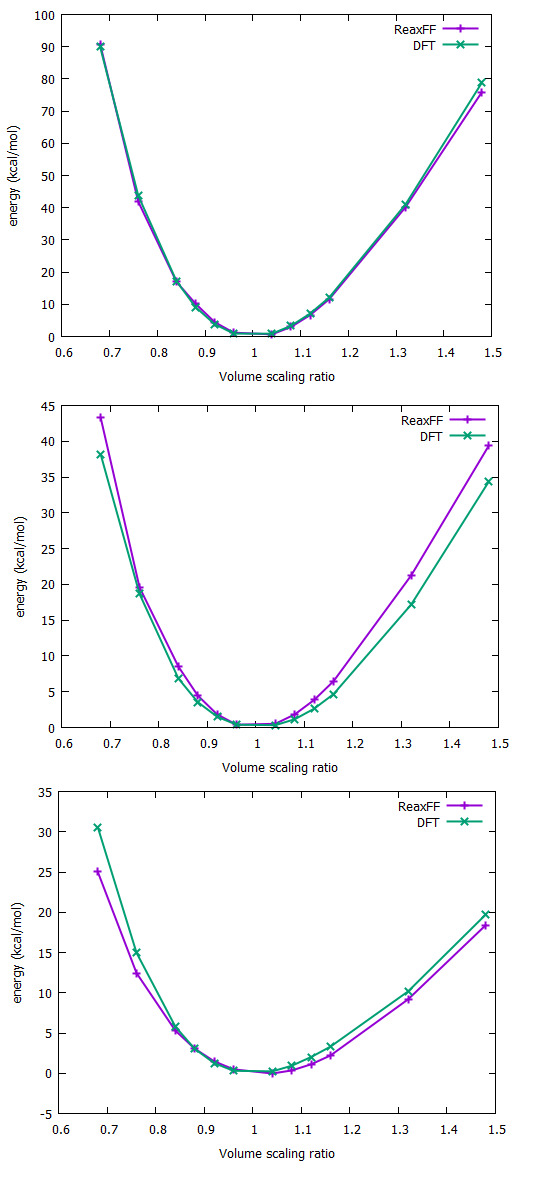
\includegraphics[scale=0.5]{Paper/images/LaEoS.png}
\caption{Calculated equations of state corresponding to crystalline La in hexagonal (top), fcc (middle), and bcc (bottom) forms.}
\label{fig:laeos}
\end{figure}

\pagebreak

\begin{figure}[hbtp]
\centering
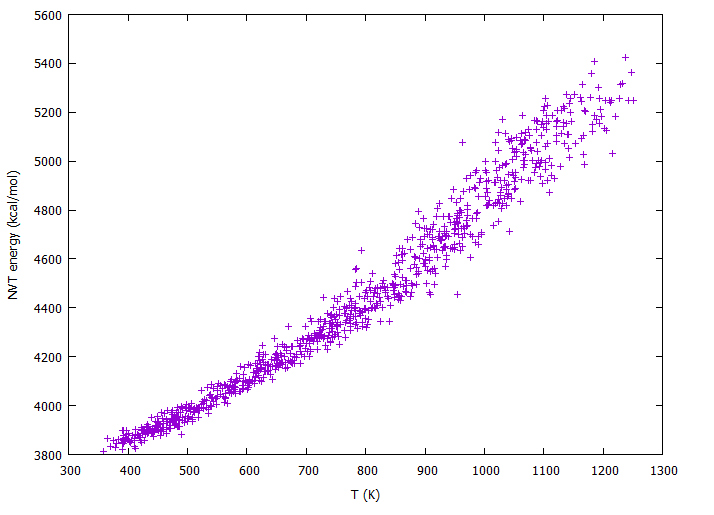
\includegraphics[scale=0.75]{Paper/images/La-nvt-EvsT.png}
\caption{Equation of state of La. Three distinct changes in slope at 550 and 1134 K indicate changes into a different crystalline structure.}
\label{fig:la-nvt-EvsT}
\end{figure}

\pagebreak

\begin{figure}[hbtp]
\centering
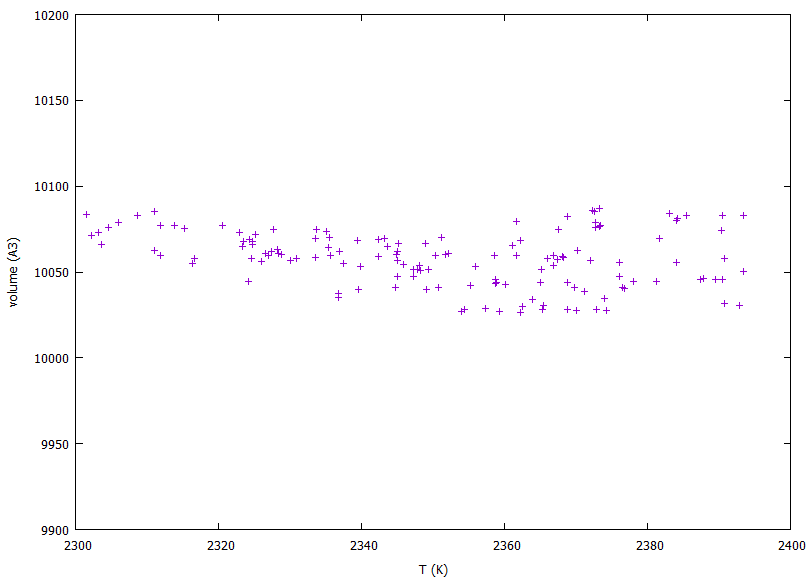
\includegraphics[scale=0.75]{Paper/images/La2O3-VvsT.png}
\caption{Equation of state of La$_2$O$_3$. According to estimated data, changes in volume at 2313 and 2383 K correspond to the changes in the crystalline structure of Lanthanum oxide.}
\label{fig:la2O3-npt-VvsT}
\end{figure}

\pagebreak

\begin{figure}[hbtp]
\centering

\includegraphics[scale=0.75]{Paper/images/placeholder.png}
\caption{La$^{3+}$--(OH$_2$)$_n$ clusters. Some bond distances obtained via DFT are highlighted and the values obtained from ReaxFF are presented in parethesis.}
\label{fig:LaOH2clusters}
\end{figure}

\pagebreak

\begin{figure}[hbtp]
\centering

\includegraphics[scale=0.75]{Paper/images/placeholder.png}
\caption{Snapshot showing La crystal structure at a temperature where (a) the packed hexagonal structure is predominant, and (b) the fcc structure is predominant. (c) Radial distribution functions showing the differences between the packed hexagonal and fcc structure of La}
\label{fig:La-alpha-gamma-RDF}
\end{figure}

\pagebreak

\begin{figure}[hbtp]
\centering

\includegraphics[scale=0.75]{Paper/images/placeholder.png}
\caption{Evolution of the radial distribution function from packed hexagonal to fcc structure with respect to temperature for La}
\label{fig:LaRDFevolution}
\end{figure}

\pagebreak

\begin{figure}[hbtp]
\centering

\includegraphics[scale=0.75]{Paper/images/placeholder.png}
\caption{Snapshot showing La$_2$O$_3$ crystal structure at a temperature where (a) the cubic, and (b) the hexagonal structure is predominant. (c) Radial distribution functions showing the differences between the two diffent structures of the La$_2$O$_3$ crystal}
\label{fig:La2O3-A-C-RDF}
\end{figure}


\pagebreak

\begin{figure}[hbtp]
\centering

\includegraphics[scale=0.75]{Paper/images/placeholder.png}
\caption{Evolution of the radial distribution function from hexagonal to cubic structure with respect to temperature for La$_2$O$_3$}
\label{fig:La2O3RDFevolution}
\end{figure}

\pagebreak
\bibliography{co2perov2}

\pagebreak
\begin{tocentry}
\begin{center}
%\includegraphics{toc.eps}
insert ToC if requested
\end{center}
\end{tocentry}


\end{document}